\documentclass[12pt,a4paper]{article}
\usepackage{hyperref}

\title{HP model for protein folding: an overview and some applications} 
\author{Gregorio Berselli, Isacco Faglioni}
\date{\today}

\usepackage{amsmath}
\usepackage{amsfonts}
\usepackage{amssymb}
\usepackage{amsthm}
\usepackage{braket}
\usepackage[margin=3cm]{geometry}
\usepackage{pgfplots}
\pgfplotsset{compat=1.18}
\usepackage{fancyhdr}
\usepackage{physics}
\usepackage{systeme,mathtools}
\usepackage{graphicx}
\usepackage{float}
\usepackage{relsize}
\usepackage{calligra}
\usepackage{siunitx}
\usepackage[miktex]{gnuplottex}
\usepackage{epstopdf}
\usepackage[english]{babel}
\usepackage{csquotes}
\usepackage{float}
\floatplacement{figure}{H}
\usepackage{tikz}
\usetikzlibrary{shapes.misc}
\usepackage[style=ieee]{biblatex}
\addbibresource{biblio.bib}
\usepackage{pgf}
\usepackage{placeins}
\usepackage{caption}
\usepackage{subcaption}

\begin{document}

\maketitle
\begin{center}
	\url{https://github.com/Grufoony/HP_model}
\end{center}

\begin{abstract}
Purpose of this project is to provide the reader with a general view of the HP model for protein folding.
Firstly, the report will focus on an overview of proteins and, in particular, why it's important to study how they fold.
Next, the HP model will be presented in its mathematical form, introducing the two main approaches to this problem: the PERM algorithm and the Deep Reinforcement Learning technique.
Then, some example of application of the PERM algorithm will be reported, obtaining results perfectly compatible with the well known benchmarks.
Lastly, a brief discussion of the results is given, together with a global resume on the whole topic.
\end{abstract}
\thispagestyle{empty}

\newpage
\thispagestyle{empty}
\addtocounter{page}{-2}
\mbox{}

\tableofcontents
\pagebreak

\section*{Introduction}
Chain molecules are a typical problem of statistical mechanics \cite{statisticalmechanics}.
The main mathematical approach applied to chain molecules is the statistical mechanics framework, which usually applies statistical methods and probability theory to large assemblies of microscopic entities.
In our case, the chain represent the system, and we're interested in the interaction within its parts.
If we set up the problem considering the system in a canonical ensemble, which means that it can exchange energy with the universe but matter, we can write the \emph{partition function} as
\begin{equation*}
    Z = \sum_i e^{-\beta\epsilon_i}
\end{equation*}
where $\epsilon_i$ is the energy of the $i$-th microstate and $\beta = \frac{1}{k_BT}$.
From that we can define the \emph{Helmholtz' free energy} of the system
\begin{equation*}
    F = -\frac{1}{\beta} \ln Z
\end{equation*}
and we know that the stable conformation of the chain will minimize this energy.
The consequence of that approach is that if we knew all the microstates (possible conformations of the chain) of the system and their energies, we would be able to compute all thermodynamic potentials.
Unfortunately, we are not able to compute every single microstate with its energy for long protein: the best we can do, as we will see, is to estimate the number of possible folds or try to find the global minima (solution) of the free energy.

In particular, this project will focus on the protein folding problem.
How protein folds is a vital process that can be useful for a lot of purposes, from bioengineering to the medical applications.
Understanding how proteins fold may help us to cure diseases like Alzheimer or anemia, in which proteins start to not fold correctly, treat virus infections and design more efficient drugs \cite{PERM}. 
Moreover, having a tool which allows us to simulate the folding process can be useful in order to understand what happens when a mutation occurs in a protein.
The reasons for mutations may be a lot, including the radiation exposure and the environment itself \cite{zanichelli}.
A mutation is not always a bad thing because evolution starts from them, and we may also force some mutations in laboratory in order to get a specific result.

The aim of this project is to report the main results in the developing of the HP model for protein folding.
In order to do so, we'll first illustrate what the HP model is.
Next, we will analyze two main approaches to this problem.
The first one is a \emph{brute force} approach, that allows us to understand the properties of a protein by computing all its possible configurations.
However, a brute force approach is typically the last thing one would do.
An alternative will be the Reinforcement Learning method that using the so-called \emph{Deep Neural Networks} (DNNs) it's able to find the minimum of the free energy in a tolerable amount of time.
\pagebreak

\section{Proteins}
Proteins are large biomolecules formed by one or more chains of amino acids.
The genetic information contained in the DNA only specifies the sequence of these amino acids, the so-called \emph{primary structure} of the protein.
It has been experimentally observed that purified proteins, i.e. proteins purified away from other cellular components, tends to spontaneously refold after being completely unfolded \cite{ProteinFolding1990}.
Understanding why and how protein folds may be a vital task for biological researches.
In fact, in order to be biologically active, a protein must adopt specific folded three-dimensional structures.
The main observable to look for in order to extract some information about protein folding is the free energy of the protein itself.
We can distinguish between three main conformational states of a protein.

\subsection{Unfolded state}
The first state we're going to discuss is the \emph{unfolded} state.
The ideal unfolded protein is the random coil, where all conformations have comparable free energies except when atoms of the polypeptide chain come into proximity.
The number of possible conformations for a protein grows exponentially with its length: it would therefore be impossible for a fully unfolded protein to encounter on a finite timescale all its possible conformations.
Consequently, the native conformation is unlikely to be found by a totally random process.

\subsection{Intermediate state}
It has been experimentally observed that many proteins exist, under certain conditions, in stable conformations that are not completely folded nor completely unfolded.
We call these states \emph{intermediate} states.
This may be caused by the free-energy landscape of the protein itself, that contains many local minima, as we can see from Fig. \ref{fig:energy_landscape}.

\begin{figure}[H]
    \centering
    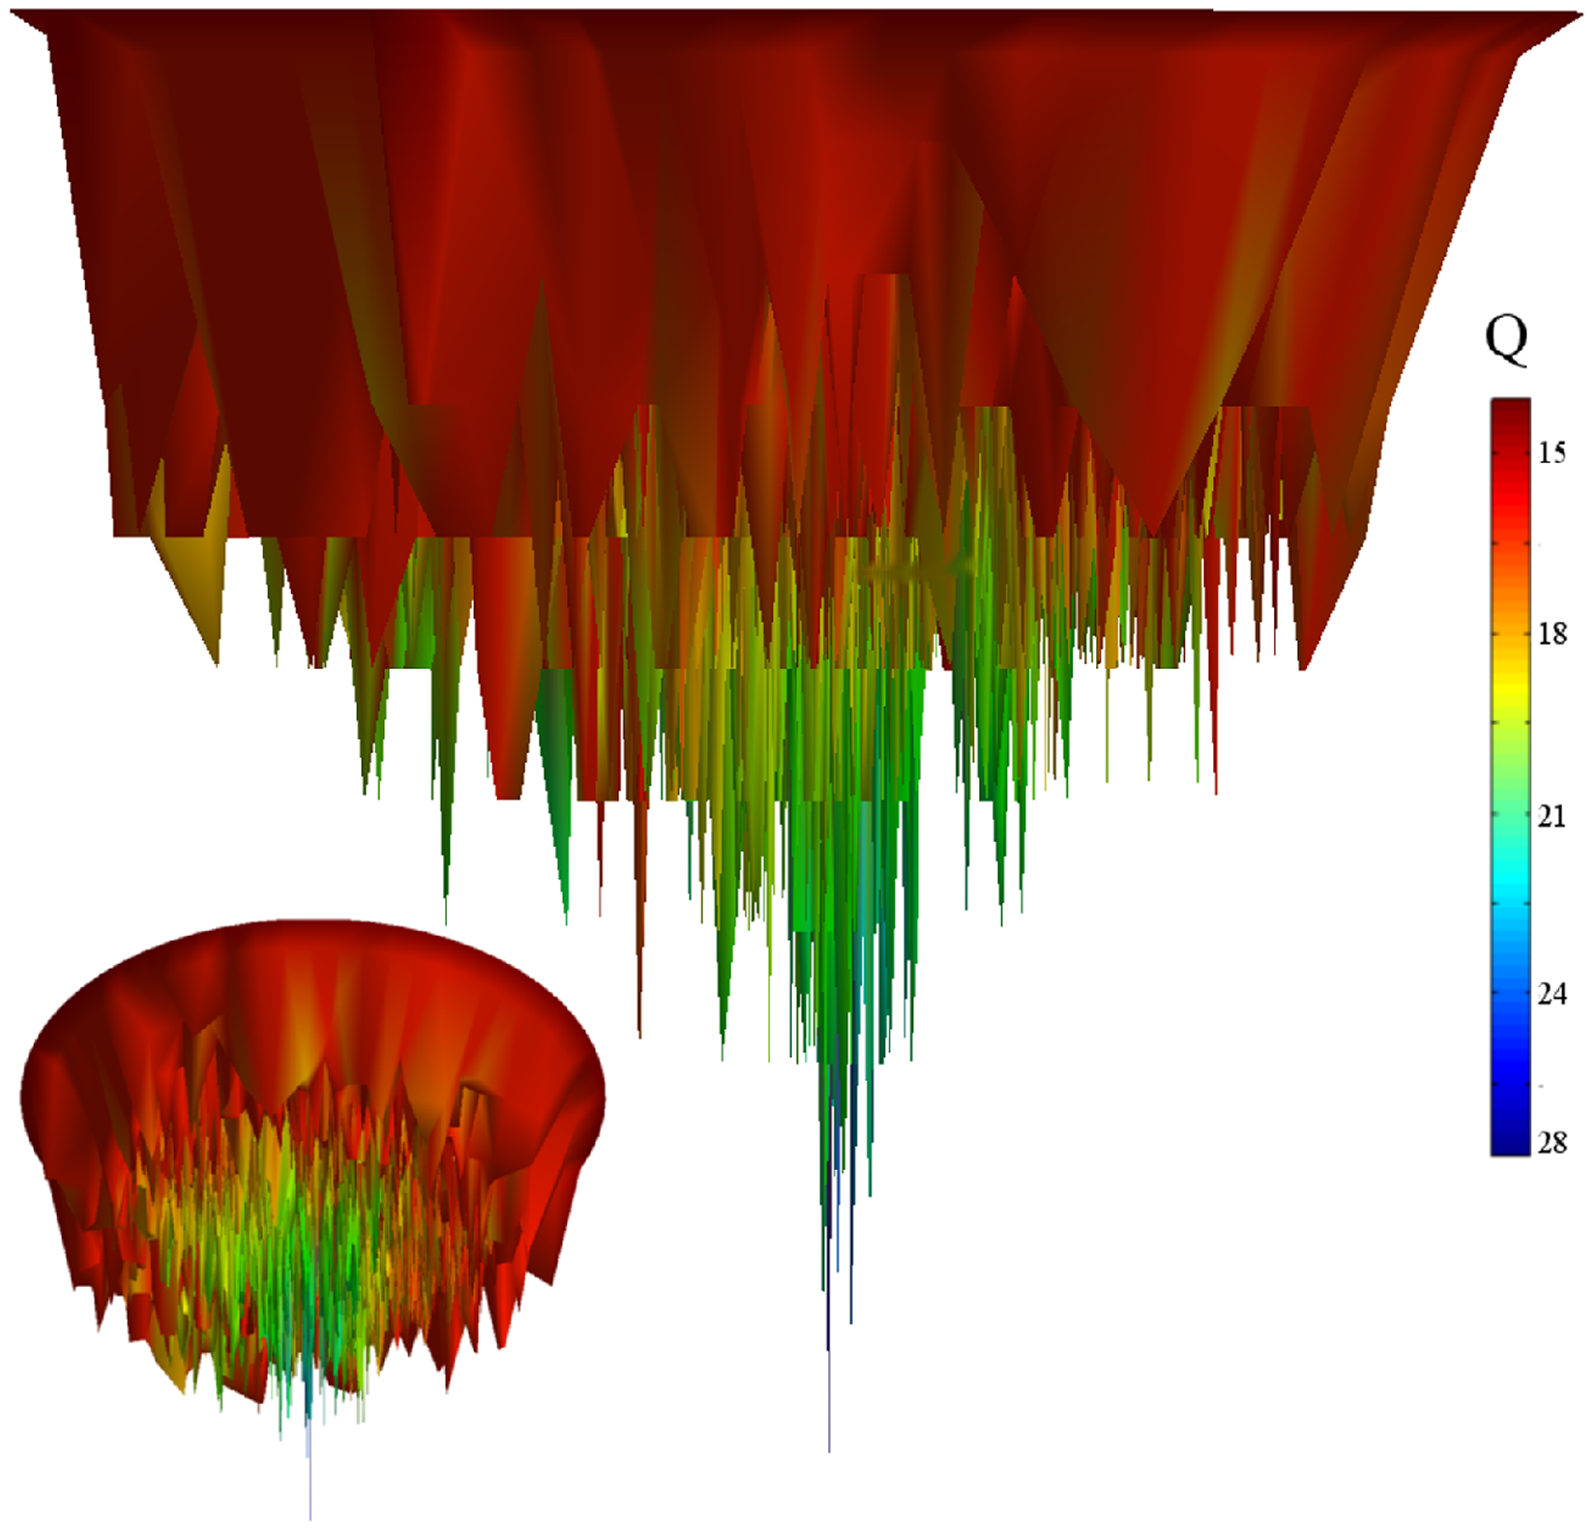
\includegraphics[width=.75\textwidth]{./img/energy_landscape.png}
    \caption{\emph{Example of a protein's energy landscape taken from \cite{energyLandscape}.
                The third axis (depth) of the funnel is associated with the energy of the local minima, and the color map represents the reaction coordinate Q.
                It's possible to see a lot of minima that are not the global one.}}
    \label{fig:energy_landscape}
\end{figure}

\subsection{Native state}
We call \emph{native} state the conformational state in which the protein is fully folded, i.e. in its (global) free-energy minimum.
The native conformations of proteins are known in great detail from the structures determined by X-ray crystallography.
How much alteration is necessary before a protein no longer folds to its normal conformation, either remaining unfolded or in an intermediate state, is not certain.
Proteins have been found to be surprisingly adaptive to mutations that would be expected to be disruptive, but the hydrophobic core seems to be the most critical aspect for stability of the normal folded state.
This criticality is the basis of HP model that we'll discuss later.

\subsection{Stability of the folded state}
Calling $\left[\text{U}\right]$ the concentration of unfolded proteins and $\left[\text{N}\right]$ the concentration of proteins in their native state, from the detailed balance we can say that
\begin{equation*}
    \left[\text{U}\right]k_\text{N} = \left[\text{N}\right]k_\text{U}
\end{equation*}
Then, it must exist an equilibrium constant $k_\text{eq} = \frac{\left[\text{N}\right]}{\left[\text{U}\right]} = \frac{k_\text{N}}{k_\text{U}}$ such that the free energy at equilibrium is
\begin{equation}
    \Delta G = G_{\text{N}} - G_{\text{U}} = k_BT\ln k_\text{eq}
    \label{eq:free_energy}
\end{equation}
The large heat capacity change upon protein unfolding causes there to be a temperature at which stability of the folded state is at a maximum: the stability of the folded state decreases at both higher and lower temperatures.

Despite this definition, it is clear that the folding problem has an aspect more similar to
\begin{equation*}
    \text{U} \leftarrow fast \rightarrow \text{I} \leftarrow slow \rightarrow \text{N}
\end{equation*}
where we've also to consider the intermediate state.
Assuming that we start from the unfolded state, there will be only one fast process from that state to an intermediate or the native one.
In this case, we can neglect the fast process and consider only the slower one and the detailed balance becomes
\begin{equation*}
    \left[\text{I}\right]k_\text{N} = \left[\text{N}\right]k_\text{I}
\end{equation*}
with a free energy analog to the Eq. (\ref{eq:free_energy}), with $k_\text{eq} = \frac{\left[\text{N}\right]}{\left[\text{I}\right]} = \frac{k_\text{N}}{k_\text{I}}$.
\pagebreak

\section{The Hydrophobic-Polar model} \label{sec:model}
The Hydrophobic-Polar model is a very simple model used to analyze the protein folding phenomenon \cite{PERM}.
The goal is, like in the complex systems field, to simplify as much as possible the problem maintaining consistency with experimental data.
In this model, the 20 types of amino acids present in nature are divided into 2 classes: the hydrophobic ones, labelled by \emph{H}, and the hydrophilic (or polar) ones, labelled by \emph{P}.
So, taking a sequence of amino acids of length $k$, we need to convert it in an \emph{HP} sequence, i.e.
\begin{equation*}
    s = \left(s_1, \ldots, s_k\right) \ , \ s_i \in \left\{H, P\right\} \ \ \forall i \in \left[1,\ldots,k\right]
\end{equation*}
Once obtained the sequence we need to define in which space $\mathbb{G}$ we want to fold it.
To simplify the problem, we may think the protein folds on a square cubic lattice $\mathbb{G} = \mathbb{Z}^2$ or a three-dimensional cubic lattice $\mathbb{G} = \mathbb{Z}^3$.
We can now define a \emph{fold} as an injective mapping $f : \left[1,\ldots,k\right] \to \mathbb{G}$ and denote with $\mathcal{Z}_k$ the set of all folds with length $k$.
It is clear that at each point $f(i)$ is assigned an amino acid $s_i$.
In order to define a way to express the energy of a fold we need to choose a function that differentiates between adjacent and connected amino acids
\begin{equation*}
    \Delta\left(f(i),f(j)\right) =
    \begin{cases}
        1 \ , \ {\left\lVert f(i) - f(j) \right\rVert}_\mathbb{G} = 1 \land i \pm 1 \neq j\\
        0 \ , \ \text{otherwise}
    \end{cases}
\end{equation*}
Now, we've seen experimentally that folded proteins tends to form hydrophobic nuclei, so we set to $-1$ the energy value of a single $H$-$H$ bond, and more in general
\begin{equation*}
    \epsilon\left(s_i,s_j\right) =
    \begin{cases}
        -1 \ , \ s_i = s_j = H\\
        0 \ , \ \text{otherwise}
    \end{cases}
\end{equation*}
So the total energy of the fold $f$ is
\begin{equation*}
    \mathcal{E}(s,f) = \sum_{0 \leq i \leq j \leq k} \epsilon\left(s_i,s_j\right)\Delta\left(f(i),f(j)\right)
\end{equation*}
The goal of the \emph{HP} model is then, like most physical problems, to minimize the energy in order to find the global minimum:
\begin{equation*}
    \mathcal{E}_\text{stable} = \min_{f \in \mathcal{Z}_k} \mathcal{E}(s,f)
\end{equation*}

\pagebreak

\section{PERM approach}
It has been shown that the \emph{HP} model is a NP hard problem, so it's very difficult to fold efficiently longer protein sequences.
We will now discuss the Rosenbluth sampling method \cite{PERM}, which involves drawing successive steps of a random walk only from among acceptable points, which are points previously not visited.

\subsection{Self-Avoiding Walks}
In a random walk process on $\mathbb{G} = \mathbb{Z}^3$, each iteration consist in a step among one out of six equally likely directions.
An analogue result is valid for $\mathbb{G} = \mathbb{Z}^2$ where we can choose one out of four equally likely directions.
Our goal is to simulate the folding of a protein of length $k$ in the space $\mathbb{G}$ by doing a random walk of $k$ steps.
The first thing we can notice is that this cannot be a regular random walk process because the fold is not allowed to cross itself or back up on itself at any iteration.
The direct consequence is that each iteration of the random walk will have some constraints, e.g. all steps after the first one will have a forbidden direction (because they cannot back up).
At this point, we can define as \emph{Self-Avoiding Walk} (SAW) a lattice path that does not visit the same point more than once.
It is known that SAWs are fractals and their number on a given lattice will increase exponentially with the length \cite{madras1988pivot}.

\subsection{Estimate the number of folds}
For simplicity, let's assume that our SAW starts form the origin of our lattice.
At any iteration $m$ we will have only $w_m$ possible moves, where $w$ represents a sort of weight of our chain.
Let's call $W$ the weight of the whole fold: a fold of length $k$ will have a weight
\begin{equation*}
    W_k = \prod_{m=1}^k w_m
\end{equation*}
It is not excluded that at a certain step $m < k$ we may have no further possibilities for continuation: we then say that a \emph{non-extendable} fold of length $m$ has been formed.
Let's denote with $\mathcal{K}$ the set of all folds with length $m \leq k$.
Clearly $\mathcal{Z}_k \subset \mathcal{K}$.
We notice that the probability of picking a random fold $f_i \in \mathcal{K}$ of length $k$ is
\begin{equation*}
    \mathbb{P}\left(f_i \in \mathcal{Z}_k\right) = \prod_{j=1}^k \frac{1}{w_j} = \frac{1}{W_k}
\end{equation*}
Let's now denote with $n_y$ the number of folds $f_i$ for which $W\left(f_i\right) = y$ and the set of these elements $\mathcal{W}_y = \left\{f \in \mathcal{K} \ | \ W\left(f_i\right) = y\right\}$.
Then, for the law of large numbers
\begin{equation*}
    \frac{n_s}{n} \approx \mathbb{P}\left(\mathcal{W}_y\right)
\end{equation*}
In the same way we can notice that
\begin{equation*}
    \left\langle W \right\rangle = \frac{1}{n} \sum_{i=1}^n W\left(f_i\right) \approx \sum_f \mathbb{P}\left(f\right)W\left(f\right) = \sum_{f \in \mathcal{Z}_k} 1 = \left\lvert \mathcal{Z}_k \right\rvert
\end{equation*}
So we've found an estimator for the number of folds
\begin{equation}
    \hat{\mathcal{Z}_k} = \left\langle W \right\rangle \approx \left\lvert \mathcal{Z}_k \right\rvert
\end{equation}
Using the \emph{batch mean method} we are also able to estimate the variance of our estimator.
Subdividing the sequence of weights $W\left(f_1\right),\ldots,W\left(f_n\right)$ into $j$ blocks of length $l$ each, so $n = jl$.
Defining the mean of the $b$-th block as
\begin{equation*}
    \mu_b = \frac{1}{l} \sum_{i = (b-1)l + 1}^{bl} W\left(f_i\right)
\end{equation*}
we can define our estimator for the variance as
\begin{equation}
    \hat{\sigma} = \sqrt{\frac{1}{j} \sum_{b = 1}^j \left(\mu_b - \left\langle W \right\rangle\right)^2}
\end{equation}
\pagebreak

\section{Reinforcement learning}
Between the plethora of agorithms used to approximate the solutions of the protein folding problem, one of the most promising is Reinforcement Learning.

\subsection{Basics of Reinforcemet Learning}

RL is a kind of algorithm that is particularly effective when the program is able to interact with the system analyzed. The main structure of a RL algorithm is that of an \emph{agent} which interacts with an \emph{enviroment} and on the base of its actions gets as feedback a \emph{reward} and the new state of the enviroment. The goal of the model is to find the best \emph{policy} which is a function that returns the action that maximizes the reward at each state.

\FloatBarrier
\begin{figure} [ht!]
    \centering
    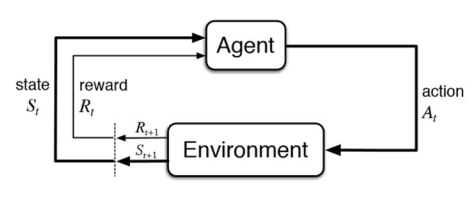
\includegraphics[scale = 0.5]{images/rl0.png}
    \caption{Basic architecture of a Reinforcement Learning algorithm}
    \label{fig:rl0}
\end{figure}
\FloatBarrier

\subsubsection{Markov Decision Processes}

MDPs are at the core of RL algorithms, since they describe a discrete-time stocastic control process. The name comes from the fact that they are an extention of the Markov chains, which are systems in which the evolution of a state depends only on the current state and not on its past. For more on the topic 
%\cite{} qua ci vuole un articolozzo


It is then necessary to descibe in Markov terms fig \ref{fig:rl0}. \emph{S} is the set of all possible states and \emph{A} is the set of all possible actions. The distribution of all possible rewards \emph{R}, can be obtained by every couple of states and actions (s, a) and for each possible adjacent couple of states there is a transition probability \emph{P} associated.

%qua sarebbe il caso di metterci una nota forse, non so bene come si faccia pero' e' una cosa che va detta pero' non penso che meriti di essere inserita nel testo
In the following paragraph we will use a common notation in RL which is that of using the capital letters to denote sets and the lowercase ones to denote single elements of the set

\subsection{Choosing optimal policies}

For each discrete instant t the system moves from a state $s_{0}$ to a state $s_{1}$ chossing an action $a$. After each action the agent recieves a reward $r$. In order to chose the optimal policy the algorithm must maximize the cumulative reward starting from a state $s_{0}$, defined as: 
\begin{equation}
\pi^{opt} = max(E(\sum_{t>0}r^{t*r|\pi}))
\end{equation}
It is worth mentioning that the expectation value has an additional constant called discount factor ($\gamma$). The expectation value for a single trajectory takes the form: $E(r) = r_{0} + \gamma r_{1} + \gamma^{2} r_{2} + ...$. From this expression it is clear that the role of the discount factor is that of giving more weight to closer rewards. This is justified due to intrinsic uncertainty that future rewards hold as a part of a MDP.

To choose in which way the algorithm should try to reach the optimal policy, the designer can choose between two different approaches:

\begin{itemize}
    \item learning through \emph{State Value} function: this function returns the sum of all rewards recieved starting from a input state following a fixed policy. Using this function one can choose the best route through states
    \item learning through \emph{Action Value} fucntion: this function returns the expected reward of taking a given action at a given state. If an algorithm uses the action value function it's called a \emph{Q-learning} algorithm    
\end{itemize}

\subsection{Q-Learning}

Q-learning is an extremely useful tool to solve the problem of non deterministic MDPs. The algorithm exploits the Q-function to associate to each state action pair a scalar value (\emph{Q-values}). Q-values are defined as the sum of all discounted rewards assuming the Agent is in state s and performs action a, and then continues playing until the end of the episode following some policy $\pi$. An optimal Q-value is a Q-value that follows the optimal policy.

\subsubsection{Bellman Equation and Optimal Q-values}

The Bellman equation for Q-learning gives the conditions for equilibrium at correct Q-values, setting therefore a constraint to optimize the policy.
\begin{equation}
Q(s_{0}, a) = r(s_{0},a ) + \gamma  max_{a'}Q(s_1, a') 
\end{equation}
$Q(s_{0}, a)$ is the Q-value associated with the couple ($s_{0}$, $a$), $r(s_{0},a )$ is the reward associated with the same couple and the term $\gamma  max_{a'}Q(s_1, a')$ is the discounted maximum Q-value for the state-action pair at the successive instant.

\subsubsection{General Q-learning algorithm}

Q-learning algorithms follow more or less the same general structure (%questo e' plagiato quindi citalo!!!!!!!):
\begin{itemize}
    \item For each pair $(s, a)$ initialize $Q(s, a)$ to 0.
    \item Repeat for each episode (complete iteration that stops at the terminal state)
    \item Select the initial state $s$.
    \item Choose a from s using policy derived from $Q$
    \item Repeat (for each step of the episode)
    \item Take action $a$, observe $r$, $s_{0}$ 
    \item Update table entry: $Q(s,a) \leftarrow r(s,a) + \gamma max_{a_{0}}Q(s_{0},a_{0})$
    \item $s \rightarrow{} s_{1}$ until new $s$ is terminal
    \item Until the maximum number of episodes reached or the Q-values do not change
\end{itemize}

An additional parameter might be given to fix how fast the Q-values should change for each iteration. This parameter is called the \emph{Learning Rate} $\alpha \in [0,1]$. In this case the Bellman equation becomes:
\begin{equation}
Q(s_{0}, a) = (1-\alpha)Q(s_{0}, a) + \alpha(r(s_{0},a ) + \gamma  max_{a'}Q(s_1, a')) 
\end{equation}

\pagebreak

\section{Results}
Our test were performed mainly on two machines: one with an Intel® Core i7-7700 @ $3.6 \ GHz$ with $16 \ GB$ of RAM and one on an AMD® Ryzen 7 @ $3.6 \ GHz$ with $32 \ GB$ of RAM.
\subsection{PERM algorithm}
We want now to report an application of the PERM algorithm, made following the article's recipe \cite{PERM}.
The goal of this algorithm is to estimate the total number of fold and then simulate a finite number of SRCs hoping to find the energy minimum.
In the article the number of iterations is set to be $10^5$ for all proteins and the result is that they found only local minima, which are intermediate states.
Our goal is to improve these 2D simulations by increasing the number of iterations, hoping to find the real minimum reported in a famous benchmark \cite{bench}.

The first protein for which we've improved the result is $HH(P)^5HH(P)^3H(P)^3HP$, that has a length of 18 amino acids (see Fig. \ref{fig:18_1}).
In particular, we've found $(1.25 \pm 0.35) \times 10^8$ folds with an energy minimum of -4 (a.u.), equal to the benchmark's one.
\begin{figure}[H]
    \centering
    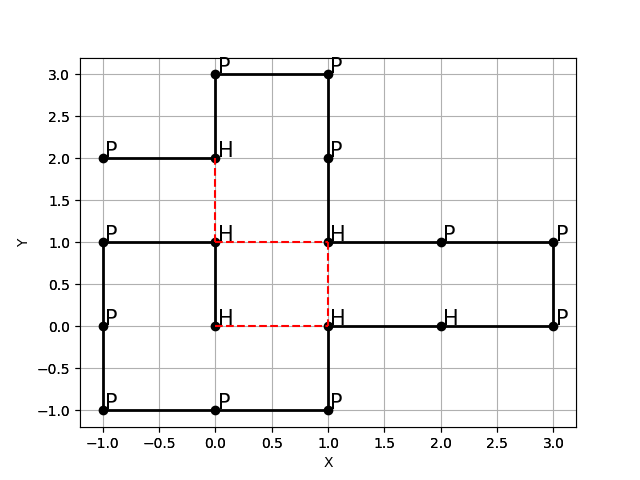
\includegraphics[width=.75\textwidth]{./img/18_1.png}
    \caption{\emph{The protein $HH(P)^5HH(P)^3H(P)^3HP$ has reached its energy minimum at -4 (a.u.) after $5 \times 10^6$ iterations ($\sim 20$ minutes).}}
    \label{fig:18_1}
\end{figure}
Another protein for which we've improved the result is $HHHP(PH)^3PP(HP)^3PH$, that has a length of 20 amino acids (see Fig. \ref{fig:20_2}).
In this case, we've found $(8.9688 \pm 0.0033) \times 10^{10}$ folds with an energy minimum of -9 (a.u.), one unit more than the benchmark's one.
\begin{figure}[H]
    \centering
    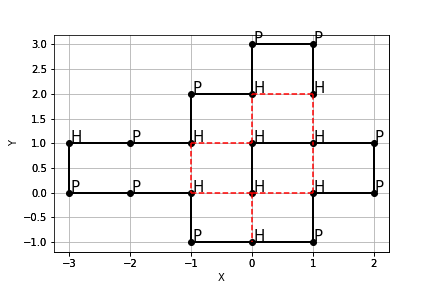
\includegraphics[width=.75\textwidth]{./img/20_2.png}
    \caption{\emph{The protein $HHHP(PH)^3PP(HP)^3PH$ has reached an energy minimum of -9 (a.u.) after $10^7$ iterations ($\sim 45$ minutes).}}
    \label{fig:20_2}
\end{figure}
We've also tried to improve the protein $HPHPHHH(P)^3HHHH(P)^2HH$, that has a length of 20 amino acids (see Fig. \ref{fig:18_2}).
However, after about 5 hours of running time it has folded with an energy of -7 (a.u.), like in the article, with an estimated number of folds equal to $(1.24 \pm 0.43) \times 10^8$.
\begin{figure}[H]
    \centering
    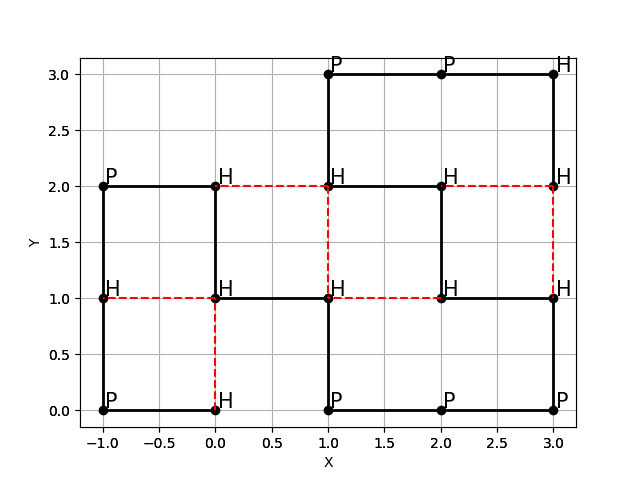
\includegraphics[width=.75\textwidth]{./img/18_2.png}
    \caption{\emph{The protein $HPHPHHH(P)^3HHHH(P)^2HH$ has reached an energy minimum of -7 (a.u.) after $10^8$ iterations ($\sim 5$ hours).}}
    \label{fig:18_2}
\end{figure}

\subsection{Constraint-based Protein Structure Prediction}
In the 2D case we showed that increasing the number of iterations resulted in better estimate of the energy.
However, the previous algorithm is not able to give significant outputs in the 3D case.
We tried so to estimate the energy in the 3D case with another algorithm, which is also based on constraint programming.
This is implemented by \emph{CPSP-tools} \cite{cpsp} and has revealed to be very powerful, folding proteins of length $\sim 200$ in few seconds.
Furthermore, this program is able to fold proteins in more complex lattices, like the 3D-face-centered-cubic one.
In our case, we wanted to improve the results of article \cite{PERM} so, in order to keep consistency, we opted for a 3D-cubic lattice.
All proteins tested converged to their minima, as we can see in Fig. \ref{fig:cpsp}.

\begin{figure}[H]
    \centering
    \begin{subfigure}[b]{0.45\textwidth}
        \centering
        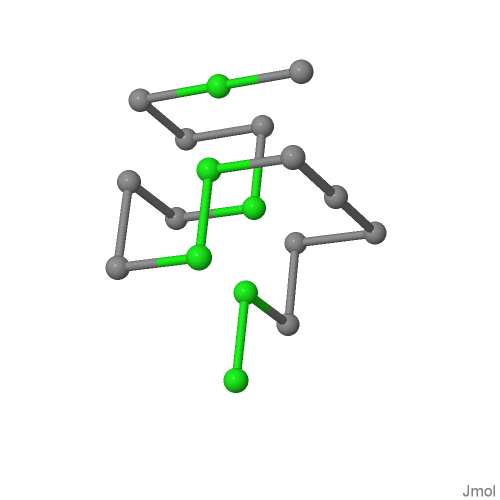
\includegraphics[width=\textwidth]{./img/18_3D.png}
        \caption{\emph{Energy $-4$ (a.u.) for the sequence $HH(P)^5HH(P)^3H(P)^3HP$.}}
    \end{subfigure}
    \begin{subfigure}[b]{0.45\textwidth}
        \centering
        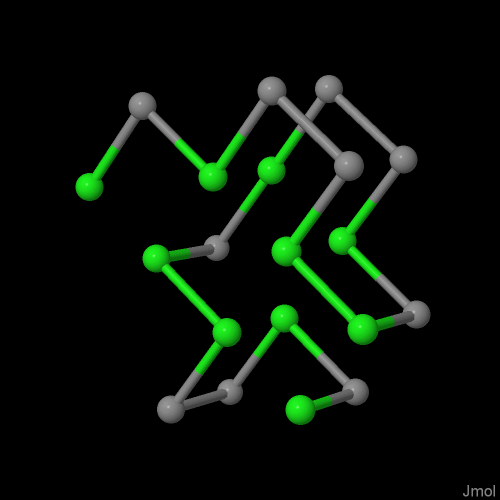
\includegraphics[width=\textwidth]{./img/20_3D.png}
        \caption{\emph{Energy $-11$ (a.u.) for the sequence $(HP)^2PH(HP)^2(PH)^2HP(PH)^2$.}}
    \end{subfigure}
    \begin{subfigure}[b]{0.45\textwidth}
        \centering
        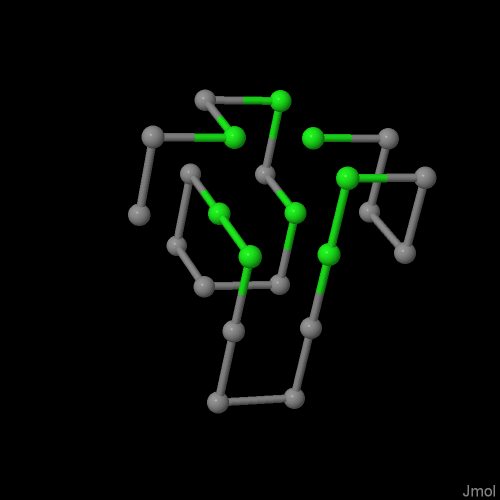
\includegraphics[width=\textwidth]{./img/24_3D.png}
        \caption{\emph{Energy $-8$ (a.u.) for the sequence $P(PH)^3(P)^4(HH(PP)^2)^2H$.}}
    \end{subfigure}
    \begin{subfigure}[b]{0.45\textwidth}
        \centering
        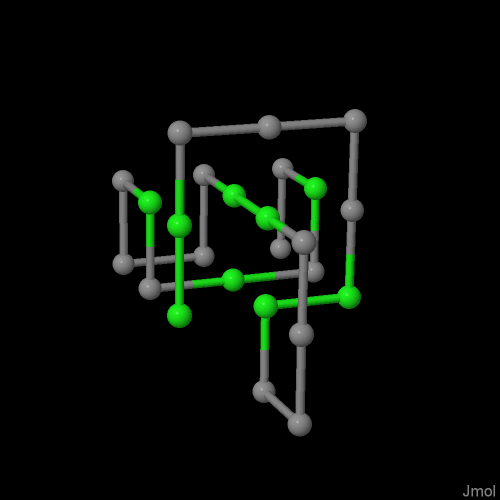
\includegraphics[width=\textwidth]{./img/25_3D.png}
        \caption{\emph{Energy $-8$ (a.u.) for the sequence $P(PH)^3(P)^4(HH(PP)^2)^2HH$.}}
    \end{subfigure}

    \caption{\emph{Four proteins of length 18 (a), 20 (b), 24 (c) and 25 (d).}}
    \label{fig:cpsp}
\end{figure}

\pagebreak

\section{Discussion}
As we saw, protein folding is actually a hard task.
The application of PERM algorithm gave better results by incrementing the number of iteration, but required a lot of computational time, e.g. 5 hours for $10^8$ iterations of Fig. \ref{fig:18_2}.
Furthermore, the application of the \emph{CPSP-tools} library managed to compute the energies in the 3D case, where the other algorithm failed.
However, this approach is not sustainable because the result's uncertainty will grow up as the protein length increases and even well-optimized brute force algorithm will suffer the curse of dimensionality.

In sec \ref{sec:RL} we explained how simple Reinforcement Learning  constitutes an \emph{smart} (AI-wise) version of the PERM algorithm, but it still falls short from a computational point of view. By comparing performances it emerged that the best models for predicting protein structure in the HP approximation are Deep Q-Networks, which are a particular kind of Reinforcement Learning algorithms that exploit neural networks. It is important to underline that despite this kind of models have already outperformed classical algorithms their research field is still thriving and there still is room for improvement

Therefore, a solution to the HP model should be searched into the Artificial Intelligence field.
Solutions based on deep reinforcement learning, and in general in the A.I. field, are more sustainable and give better results.
Bioinformatics is conceptualizing biology in terms of molecules and applying ``informatics techniques'' to understand and organize the information associated with these molecules, on a large scale \cite{bioinfo}.
The aims of bioinformatics are multiple.
Firstly, well-organized data allow researches to access existing information and to submit new entries as they are produced.
Secondly, it develops tool and resources useful for the analysis of these data.
The development of these tools requires a lot of knowledge in biology, informatic and also physics and mathematics.
\begin{figure}[H]
    \centering
    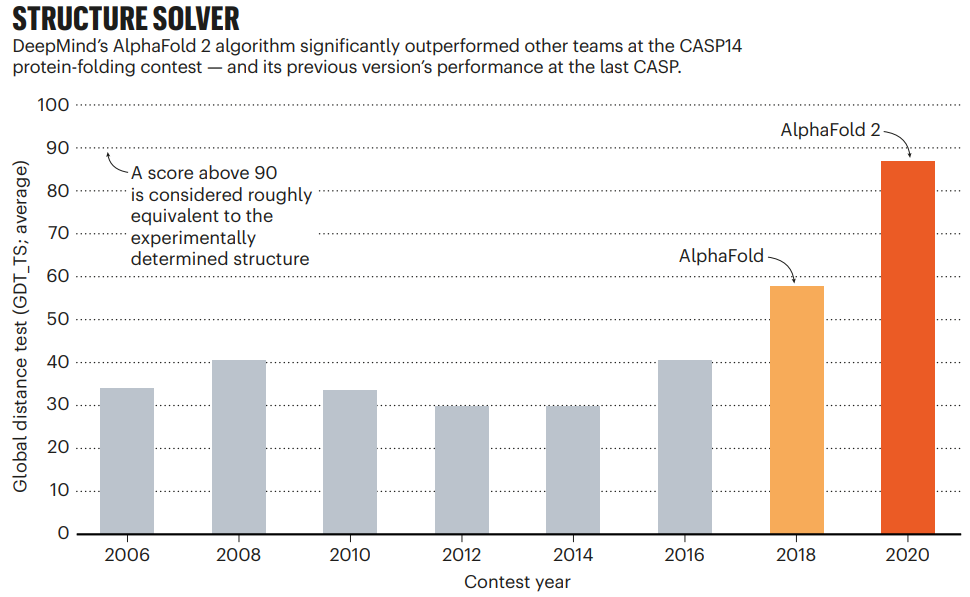
\includegraphics[width=.75\textwidth]{./img/alphafold.png}
    \caption{\emph{Protein folding algorithms' accuracy through time \cite{alphafold}.}}
    \label{fig:alphafold}
\end{figure}
Two example of intelligences that are giving many good results are AlphaFold and AlphaFold2 by Google.
In particular, the second one reached a precision level comparable to the experimental one, as wee can see from Fig \ref{fig:alphafold}.
The future of this topic seems to be linked to research whose goal is to expand the protein databases underlying these intelligences.

\pagebreak

\newpage
\thispagestyle{empty}
\mbox{}

\printbibliography

\end{document}
